%=========================================================
% 32bit ISA Code Assignments
%=========================================================
\section{32bit ISA Code Assignments}

\begin{table}[H]
    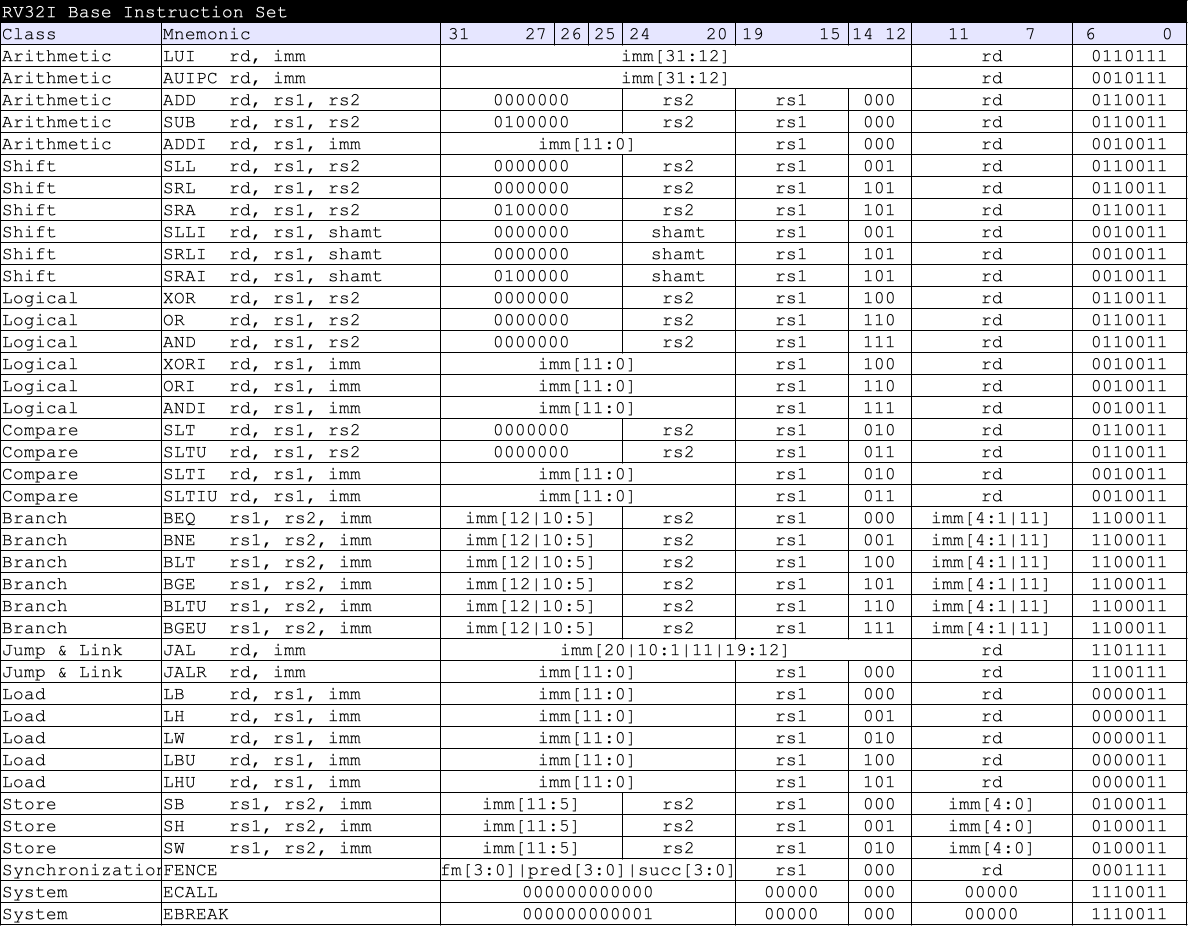
\includegraphics[width=1.00\columnwidth]{./Table/ISACode_RV32I.png}
    \caption{RV32I Base Instruction Set Code}
    \label{tb:ISACode_RV32I}
\end{table}

\begin{table}[H]
    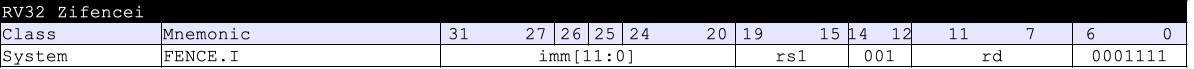
\includegraphics[width=1.00\columnwidth]{./Table/ISACode_RV32Zifencei.png}
    \caption{RV32 Zifencei Code}
    \label{tb:ISACode_RV32Zifencei}
\end{table}

\begin{table}[H]
    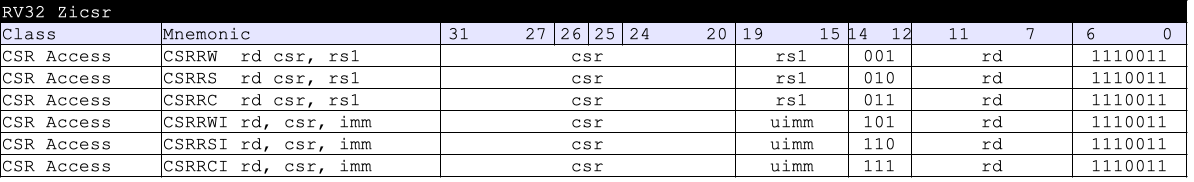
\includegraphics[width=1.00\columnwidth]{./Table/ISACode_RV32Zicsr.png}
    \caption{RV32 Zicsr Code}
    \label{tb:ISACode_RV32Zicsr}
\end{table}

\begin{table}[H]
    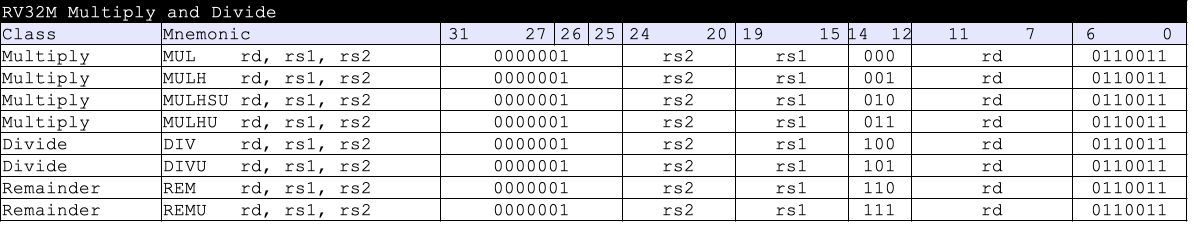
\includegraphics[width=1.00\columnwidth]{./Table/ISACode_RV32M.png}
    \caption{RV32M Multiply and Divide Code}
    \label{tb:ISACode_RV32M}
\end{table}

\begin{table}[H]
    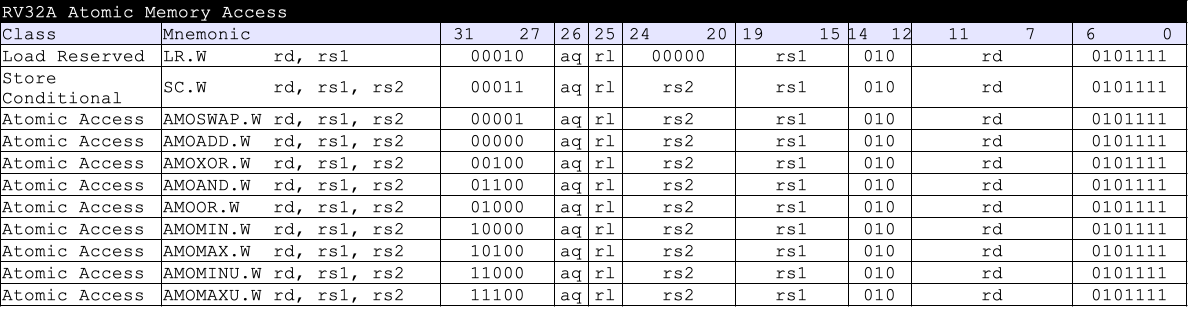
\includegraphics[width=1.00\columnwidth]{./Table/ISACode_RV32A.png}
    \caption{RV32A Atomic Memory Access Code}
    \label{tb:ISACode_RV32A}
\end{table}

\begin{table}[H]
    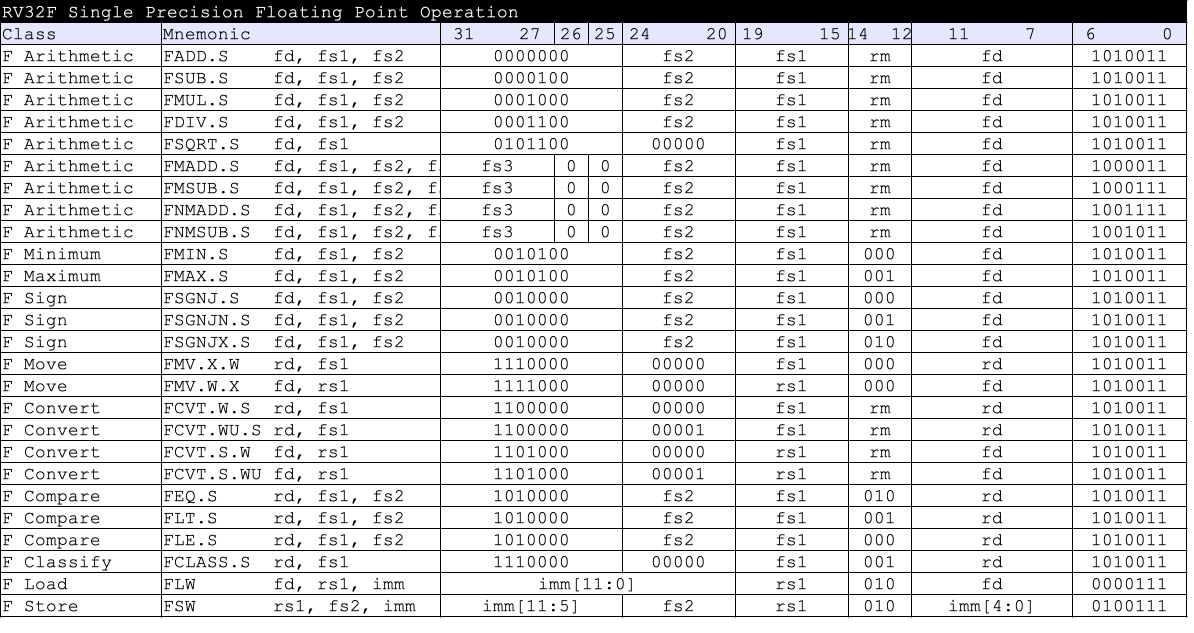
\includegraphics[width=1.00\columnwidth]{./Table/ISACode_RV32F.png}
    \caption{RV32F Single Precision Floating Point Operation Code}
    \label{tb:ISACode_RV32F}
\end{table}

\begin{table}[H]
    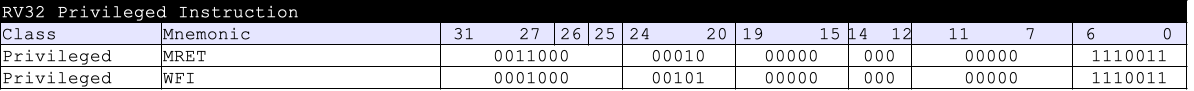
\includegraphics[width=1.00\columnwidth]{./Table/ISACode_RV32Priviledged.png}
    \caption{RV32 Privileged Instruction Code}
    \label{tb:ISACode_RV32Priviledged}
\end{table}




